\chapter{Python 概述与安装}
\section{Python 的发展历史与应用}
Python 的诞生时间非常早,第一版 Python 发行于 1991 年,甚至比 Java 的历史都早。在大部分时间内,Python 一直作为一个小众的编程语言,并没有大规模流行起来。近些年来,随着大数据技术、人工智能技术的发展和普及,“简洁、具有良好扩展性”的 Python 非常契合大数据与人工智能技术对编程语言的要求,超越其他编程语言迅速崛起。Python 分别在2010年,2018年被全球知名的编程语言流行度排行榜网站 TIOBE 评为“年度最佳编程语言”,并长期位于各年或各月流行编程语言排行榜的前三名。中国的网络上甚至产生了一句流行语:“人生苦短,我用 Python”。

Python 的创始人为荷兰人吉多·范罗苏姆(Guido van Rossum),在 1989 年的圣诞节期间,吉多·范罗苏姆为了打发时间,决心开发一个新的脚本解释程序,作为 ABC语言的继承,于是 Python 诞生了。之所以选择 Python 作为名字,是由于吉多·范罗苏姆非常喜欢一部 BBC 电视剧--- Monty Python's Flying Circus(中文译名:蒙提·派森的飞行马戏团)。 Python 的英文意思为蟒蛇,这也是为什么一些 Python 相关的软件或书籍用蟒蛇作为图标的原因。

Python的设计哲学是“优雅”、“明确”、“简单”,Python 可以说是语法功能最简单的编程语言之一。Python具有良好的可扩展性,Python提供了丰富的接口和工具,以便程序员能够轻松地使用 C、C++、Cython来编写扩展模块,因此,有很多人把Python作为一种“胶水语言”使用。Python是完全面向对象的语言,函数、模块、数字、字符串都是对象,并且完全支持继承、重载、派生、多重继承等,Python 还支持重载运算符。并且随着计算机速度运算速度越来越快,Python 运算速度慢的缺点逐渐可以忽略,因此,许多网站开始使用 Python 开发,许多专业软件也开始支持 Python 调用。

Python 的应用范围包括 Web 开发网站与网络爬虫,GUI 开发桌面软件,科学计算等。使用Python编写的著名应用包括:

\vspace{5pt}
\begin{itemize}
  \item Youtube --- 视频分享网站

  \item Dropbox --- 文件分享软件

  \item Instagram --- 图片分享软件


  \item 豆瓣网 --- 国内著名的图书、唱片、电影评论网站

  \item 知乎网 --- 国内著名的问答网站

  \item 果壳网 --- 国内著名的泛科技主题网站
\end{itemize}
\vspace{5pt}

目前的主要 Python 版本为 Python3,本书的所有 Python 程序都是 Python3 版本。

\clearpage
\section{安装 Python}

使用 Python 时一般有两种方式:一是下载 Anaconda(自带 Python,编辑器 Spyder以及许多常用包),二是下载 Python 和编辑器 Pycharm,从实践经验来看,Pycharm 功能比 Spyder 更多,对程序员来说更加便捷,但 Anaconda 对新手比较友好,很多常用包已经自动安装好了,不用自己专门再下载。若对 python 有一定经验,需要经常用 python 编写程序,推荐使用 Pycharm;若是刚刚接触 python,则推荐使用 Anaconda。

\subsection{Anaconda}

Anaconda包括Python、Spyder 以及一大堆安装好的工具包,比如:numpy、pandas、matplot、scipy,在 Anaconda 里面还可以使用 R 语言、Notebook 等。 Anaconda 下载的官方网址为:\href{https://www.anaconda.com/distribution}{https://www.anaconda.com/distribution}。点击 Downloand 选择自己操作系统的 Python 3 版本下载(本书的软件安装以 Windows 系统为例)。

\begin{figure}[!ht]
  \centering
  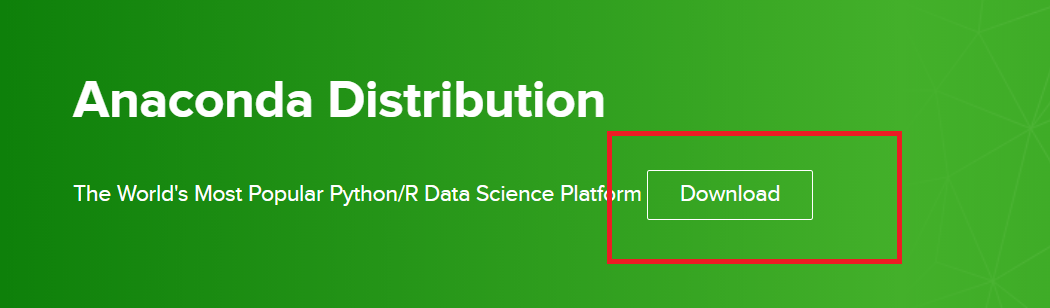
\includegraphics[scale=0.5]{figure/chapter1/anaconda.png}
\end{figure}

\begin{figure}[!ht]
  \centering
  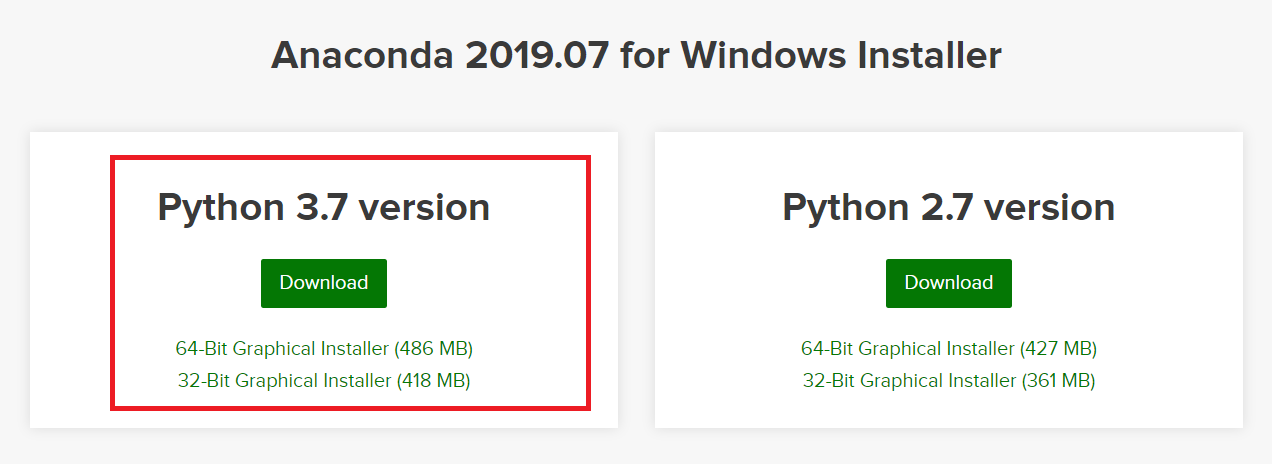
\includegraphics[scale=0.5]{figure/chapter1/anaconda2.png}
\end{figure}

下载完毕后,双击 exe 文件安装,安装过程参照下图:


\begin{figure}[!ht]
  \centering
  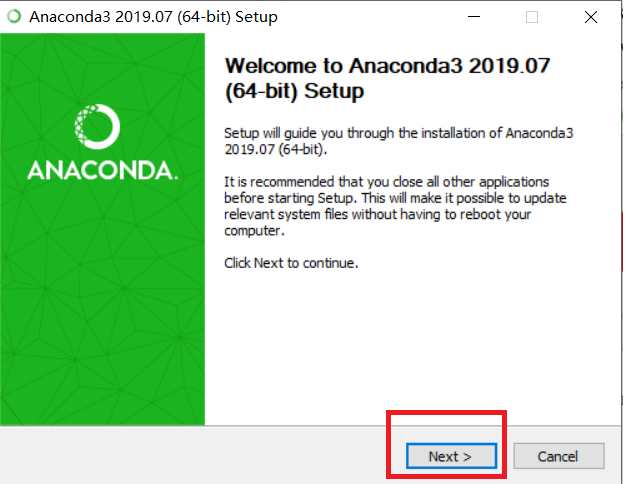
\includegraphics[scale=0.5]{figure/chapter1/anaconda7.png}\quad
  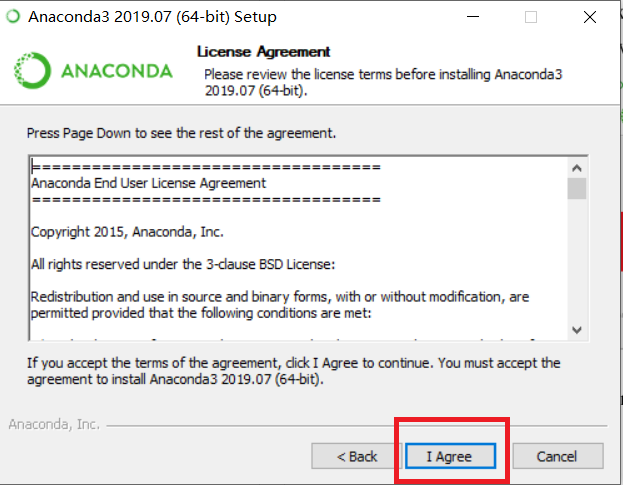
\includegraphics[scale=0.5]{figure/chapter1/anaconda8.png}
\end{figure}

安装目录默认的是 C 盘,可以通过点击 Browse 更改为自定义位置。


\begin{figure}[!ht]
  \centering
  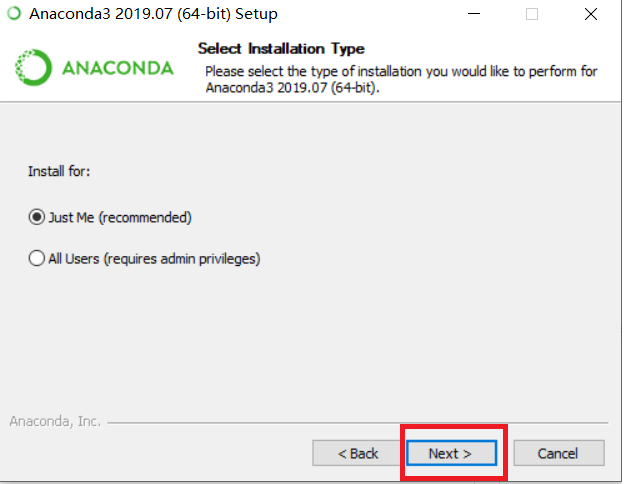
\includegraphics[scale=0.5]{figure/chapter1/anaconda9.png}\quad
  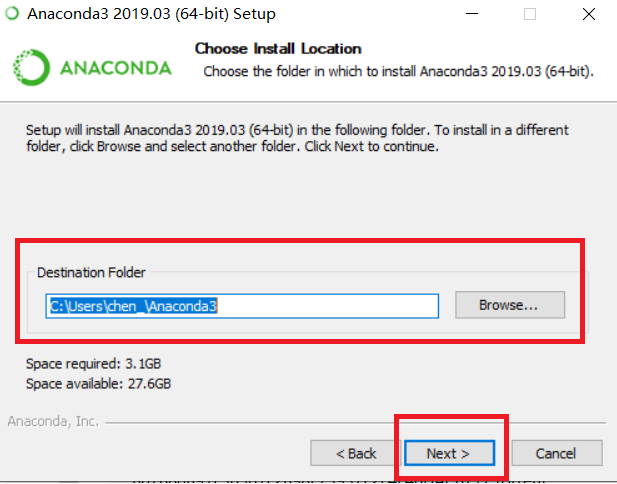
\includegraphics[scale=0.5]{figure/chapter1/anaconda3.png}
\end{figure}

\begin{figure}[!ht]
  \centering
  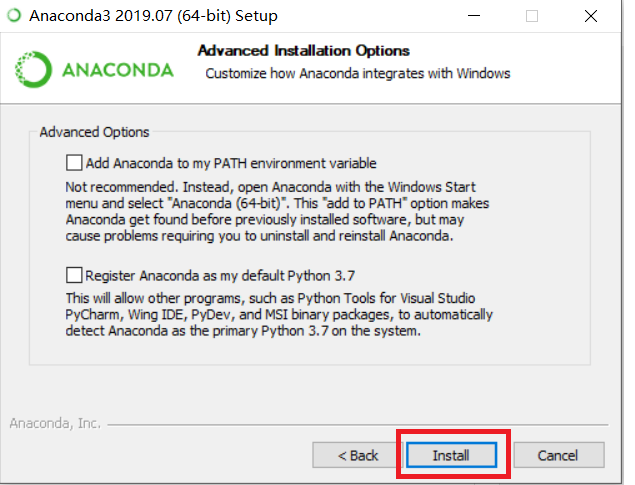
\includegraphics[scale=0.5]{figure/chapter1/anaconda10.png}\quad
  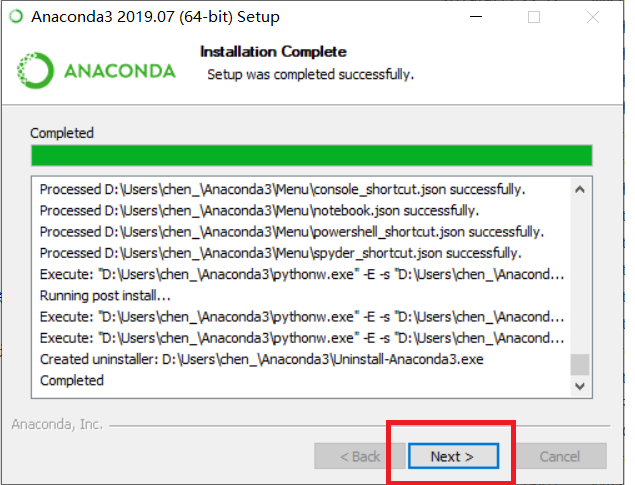
\includegraphics[scale=0.5]{figure/chapter1/anaconda12.png}
\end{figure}

\begin{figure}[!ht]
  \centering
  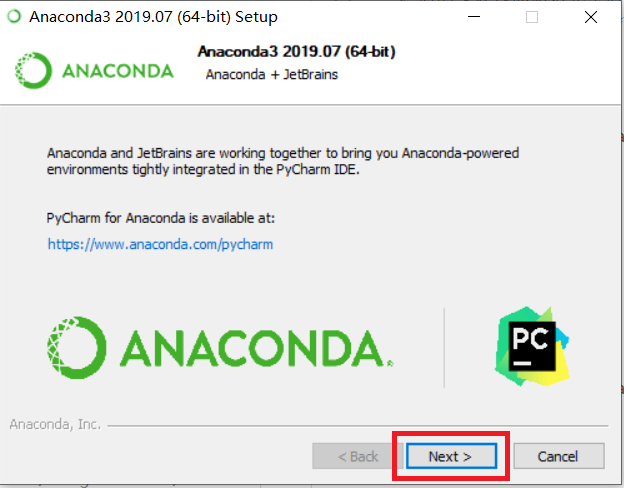
\includegraphics[scale=0.5]{figure/chapter1/anaconda13.png}\quad
  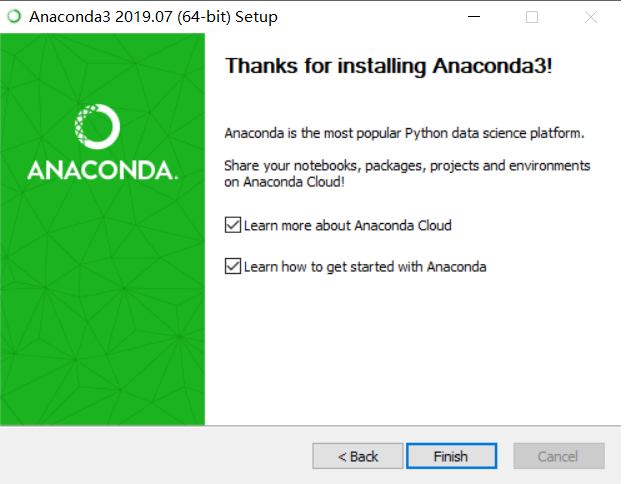
\includegraphics[scale=0.5]{figure/chapter1/anaconda14.png}
\end{figure}

安装完毕后,在 Windows 菜单栏里找到名为“Anaconda-Navigator”的图标,点击打开 Anaconda。

\clearpage
\begin{figure}[!ht]
  \centering
  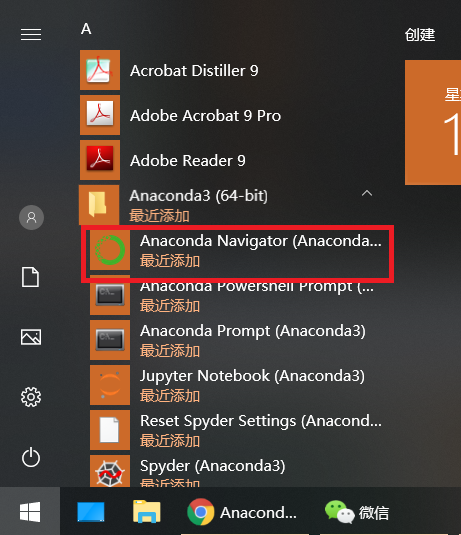
\includegraphics[scale=0.5]{figure/chapter1/anaconda11.png}
\end{figure}


启动(Launch) Spyder,就能够编译 Python 了。

\begin{figure}[!ht]
  \centering
  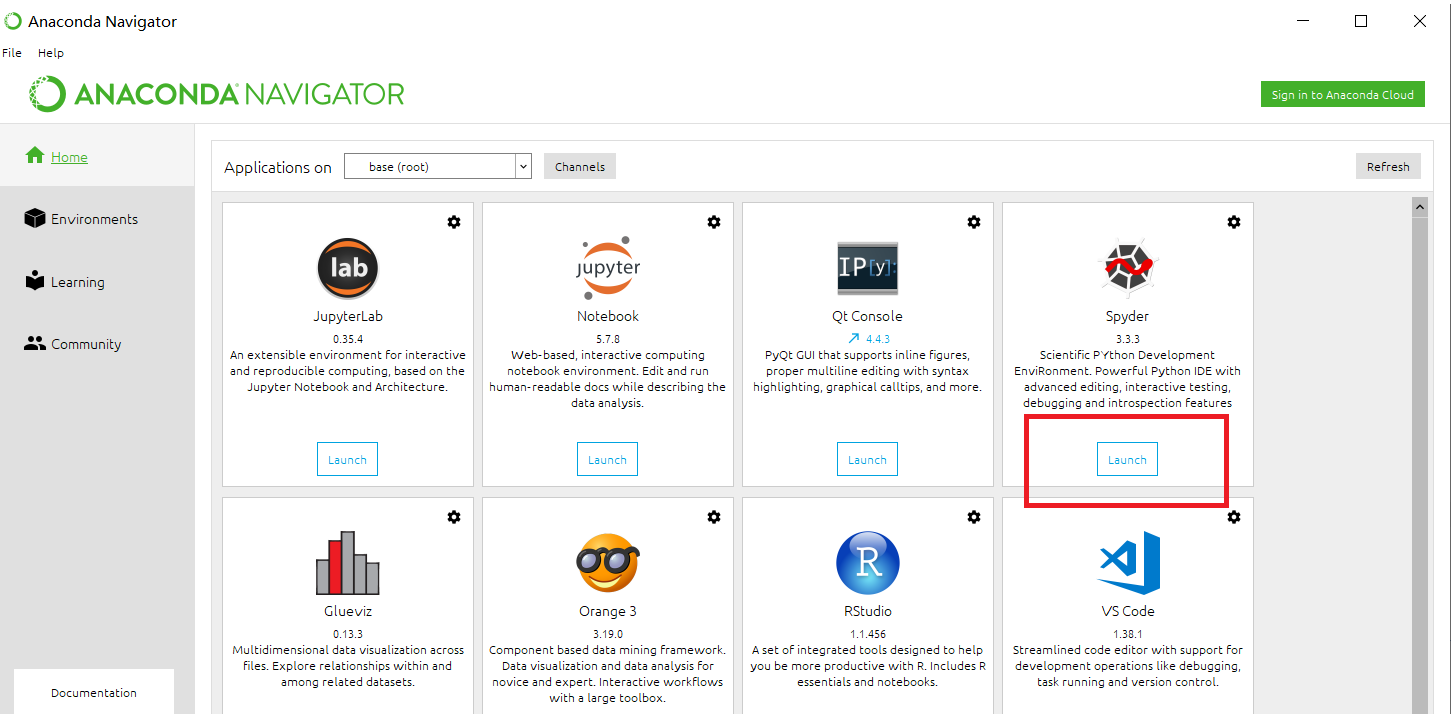
\includegraphics[scale=0.3]{figure/chapter1/anaconda4.png}
\end{figure}


Spyder 的界面非常类似 Matlab,交互式工具 Ipython console 就在窗口界面中。我们在 Ipython 中输入 print(`Hello world'),目的是让 Python 把 Hello World 打印到屏幕上,测试 Spyder的运行。

\begin{figure}[!ht]
  \centering
  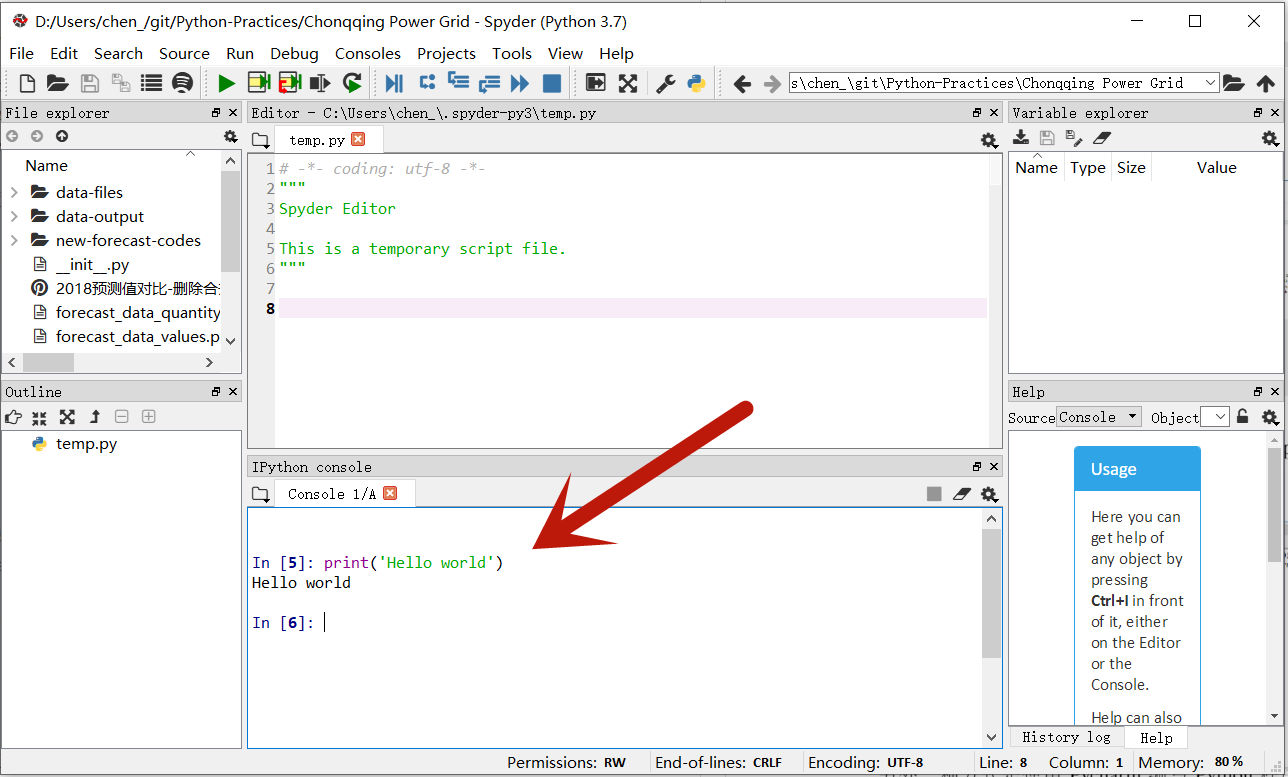
\includegraphics[scale=0.4]{figure/chapter1/anaconda5.png}
\end{figure}


\clearpage
\subsection{Python + Pycharm}

另外一种方式是使用 Pycharm 编写 Python 程序,但由于 Pycharm 并不自带 python,我们还需要专门把 python 下载下来。

\subsubsection{下载python}

Python 的官方网址为:\href{https://www.python.org}{https://www.python.org}。打开网址后,从 Download 里面可以找到不同操作系统的 python 版本下载。下面我们以 Windows 系统为例讲述 Python 的安装。

\begin{figure}[!ht]
  \centering
  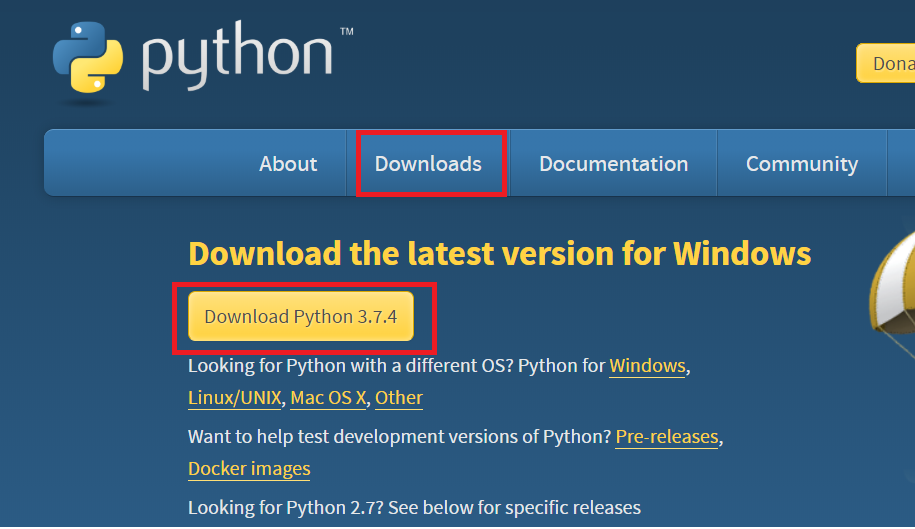
\includegraphics[scale=0.6]{figure/chapter1/pythonDownload.png}
\end{figure}

下载完成后,双击 exe 文件安装,切记要勾选 Add Python 3.7 to PATH, 然后点击 Install Now(默认安装目录,默认安装 pip 等)或 Customize installation(可以自己设置安装目录等),我们选择 Customize installation。

\begin{figure}[ht]
  \centering
  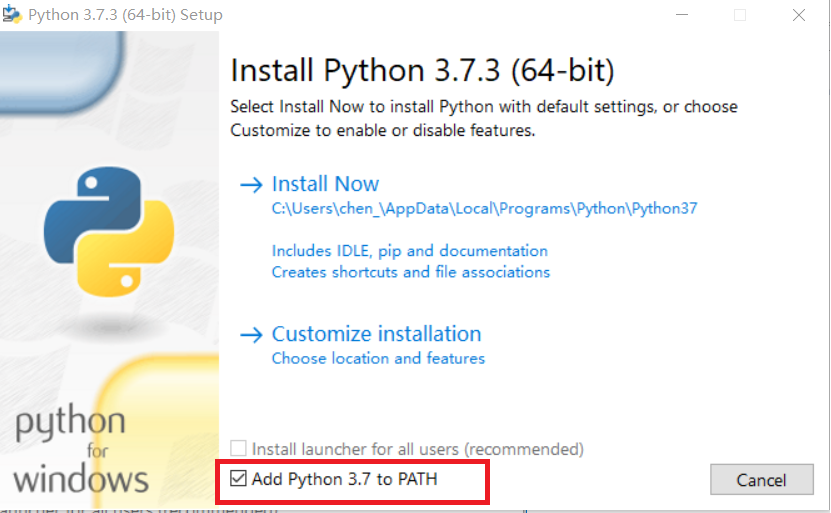
\includegraphics[scale=0.4]{figure/chapter1/pythonDownload2.png}\quad
  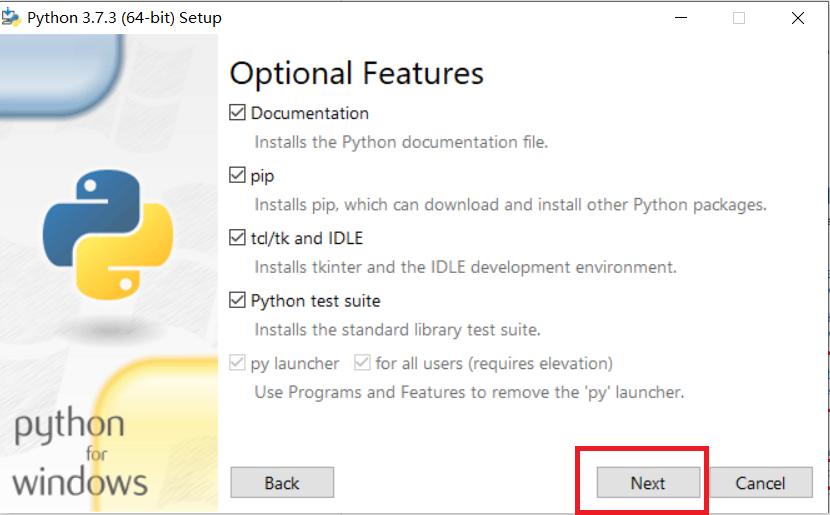
\includegraphics[scale=0.4]{figure/chapter1/pythonDownload4.png}
\end{figure}

\clearpage
\begin{figure}[ht]
  \centering
  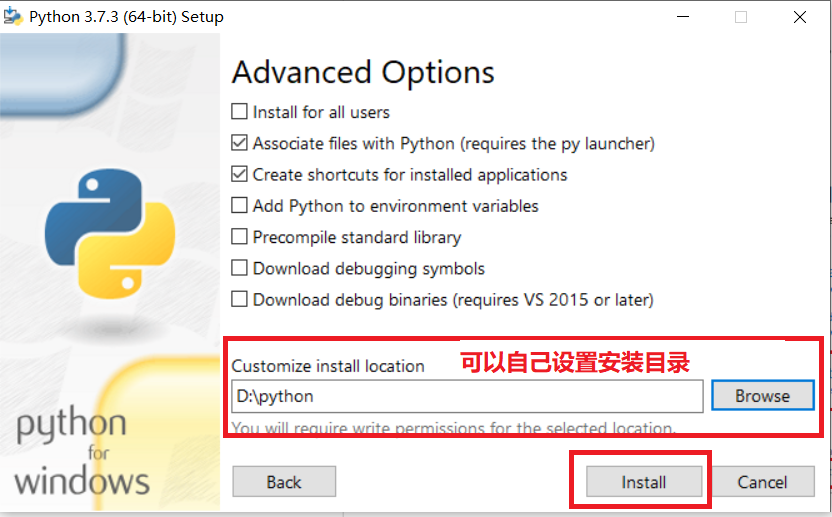
\includegraphics[scale=0.4]{figure/chapter1/pythonDownload5.png}\quad
  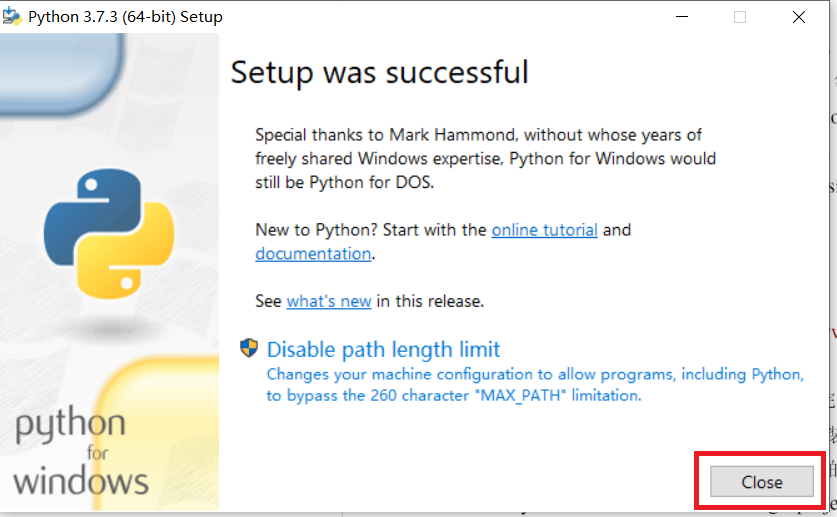
\includegraphics[scale=0.4]{figure/chapter1/pythonDownload6.png}
\end{figure}

为了测试 Python 是否安装成功,打开命令行窗口(win10 系统中敲 win 健,再输入 cmd,然后回车),输入 python -{}-version(注意是两个短横线),若能显示 Python 的版本信息,则代表 python 已正确安装。

\begin{figure}[!ht]
  \centering
  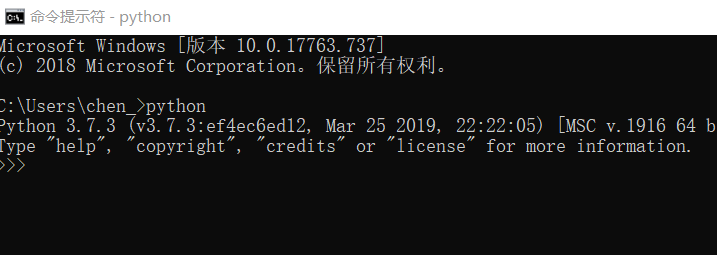
\includegraphics[scale=0.7]{figure/chapter1/pythonDownload3.png}
\end{figure}

\subsubsection{下载 Pycharm}


Pycharm 的官方网址:\href{http://www.jetbrains.com/pycharm}{http://www.jetbrains.com/pycharm},点击 DOWNLOAD 开始安装。

\begin{figure}[!ht]
  \centering
  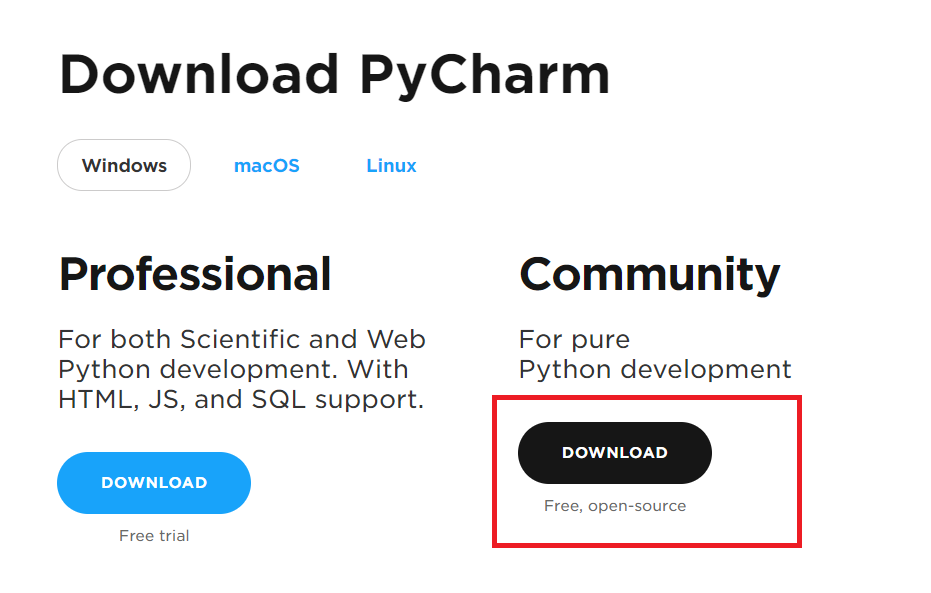
\includegraphics[scale=0.6]{figure/chapter1/pycharm.png}
\end{figure}

一般选择免费版本下载,下载完成后双击 exe 进行安装。

\clearpage
\begin{figure}[!ht]
  \centering
  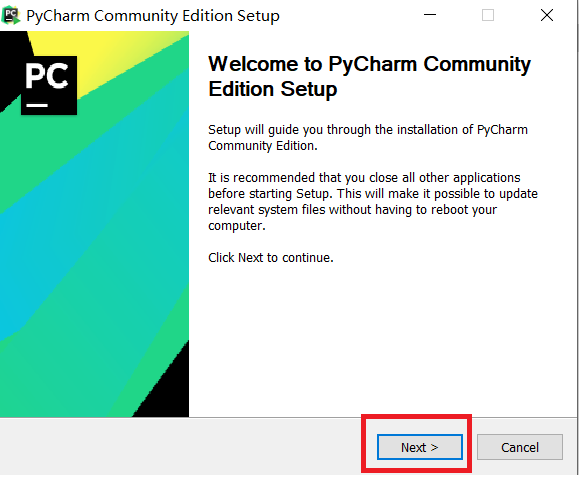
\includegraphics[scale=0.5]{figure/chapter1/pycharm5.png}\quad
  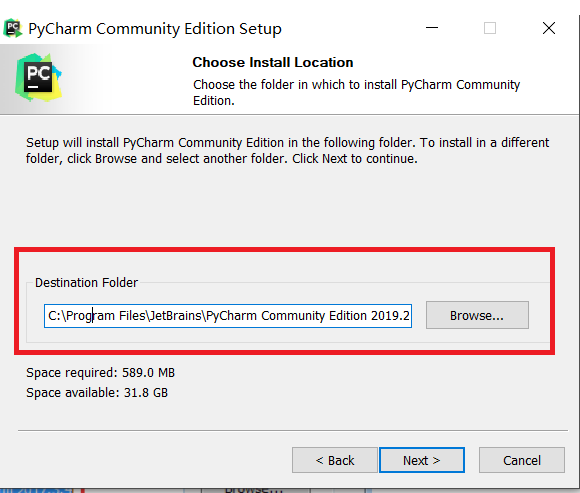
\includegraphics[scale=0.5]{figure/chapter1/pycharm2.png}
\end{figure}

可以通过图中的 Browse 更改安装目录,其他步骤按照默认设置即完成安装。
\begin{figure}[!ht]
  \centering
  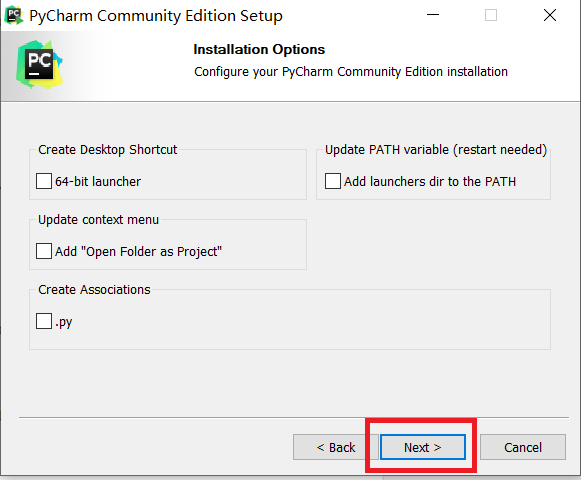
\includegraphics[scale=0.5]{figure/chapter1/pycharm6.png}\quad
  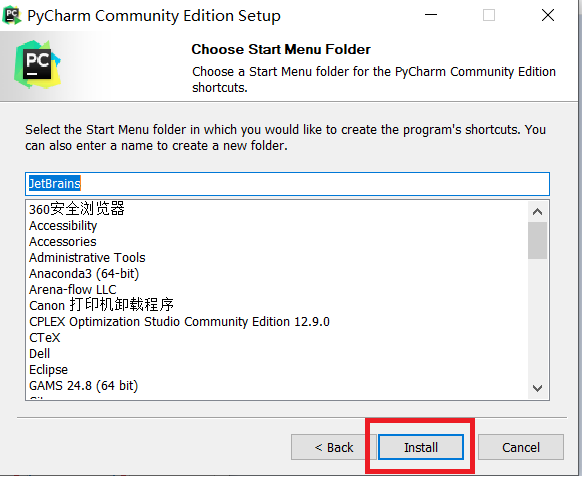
\includegraphics[scale=0.5]{figure/chapter1/pycharm7.png}
\end{figure}

\begin{figure}[!ht]
  \centering
  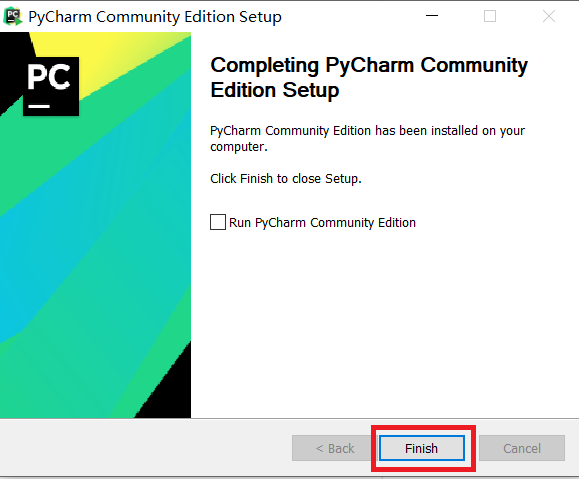
\includegraphics[scale=0.5]{figure/chapter1/pycharm8.png}
\end{figure}


完成安装后,从 Windows 菜单栏里找到 jetbrains Pycharm,点击打开 Pycharm。

\begin{figure}[!ht]
  \centering
  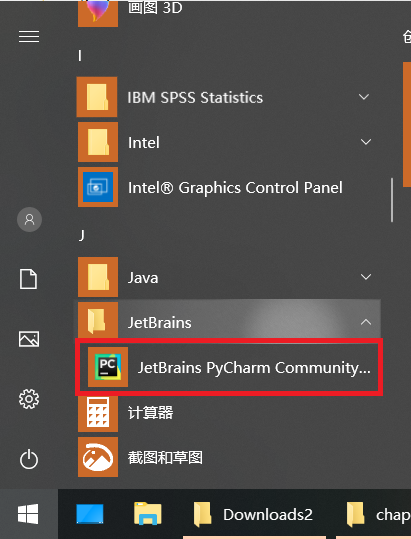
\includegraphics[scale=0.4]{figure/chapter1/pycharm9.png}
\end{figure}

之后的设置如下面的图所示:

\begin{figure}[!ht]
  \centering
  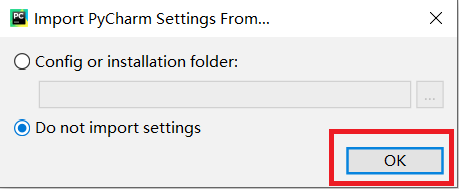
\includegraphics[scale=0.8]{figure/chapter1/pycharm10.png}
\end{figure}

\begin{figure}[!ht]
  \centering
  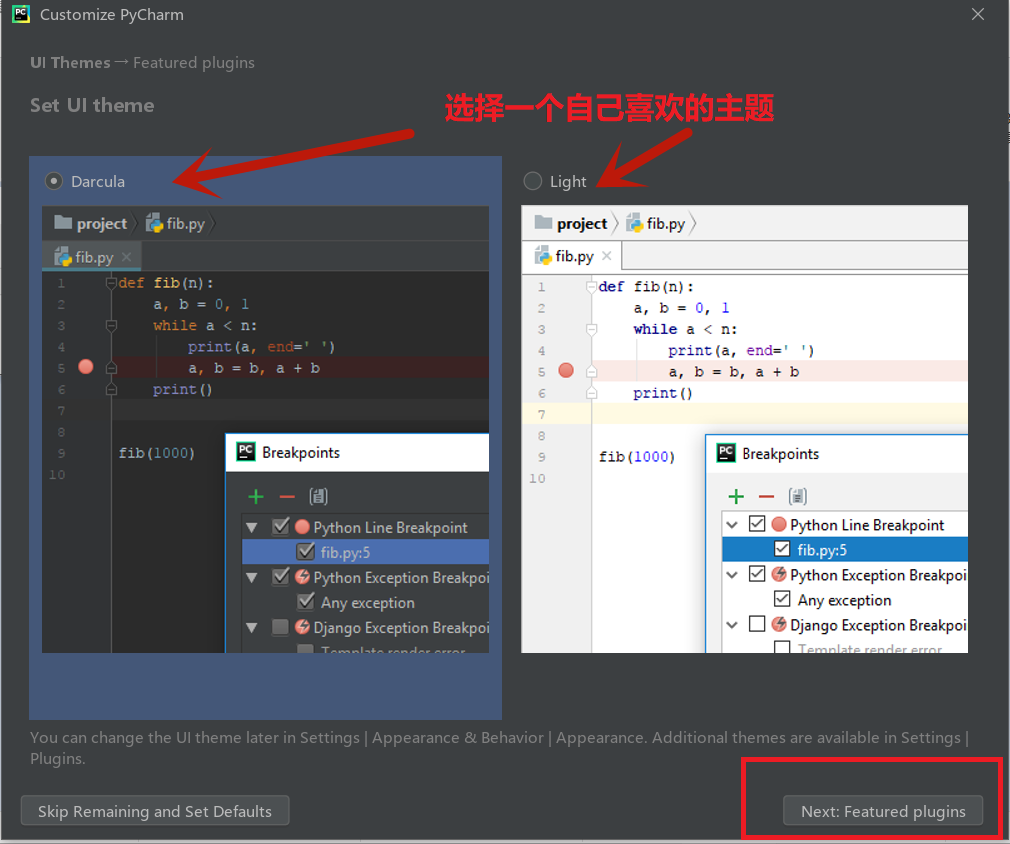
\includegraphics[scale=0.3]{figure/chapter1/pycharm11.png}\quad
  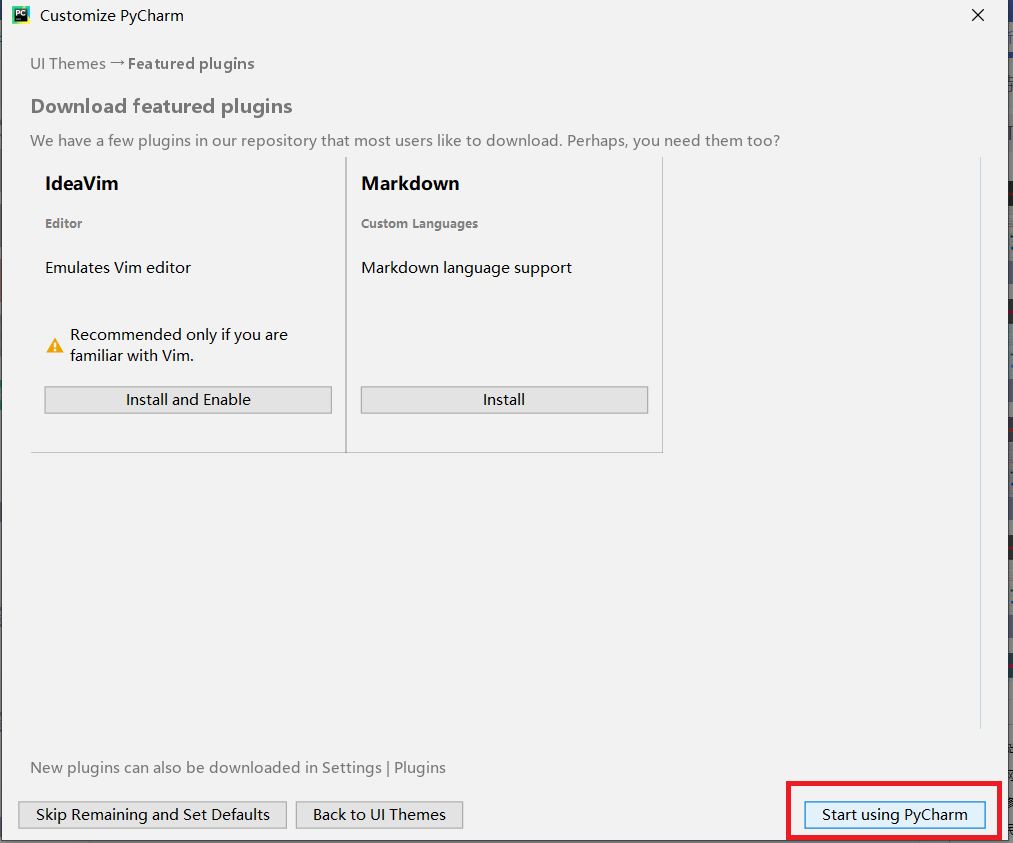
\includegraphics[scale=0.3]{figure/chapter1/pycharm12.png}
\end{figure}

点击 Create New Project,创建一个新项目,项目的地址以及名字可以自己替换。

\begin{figure}[!ht]
  \centering
  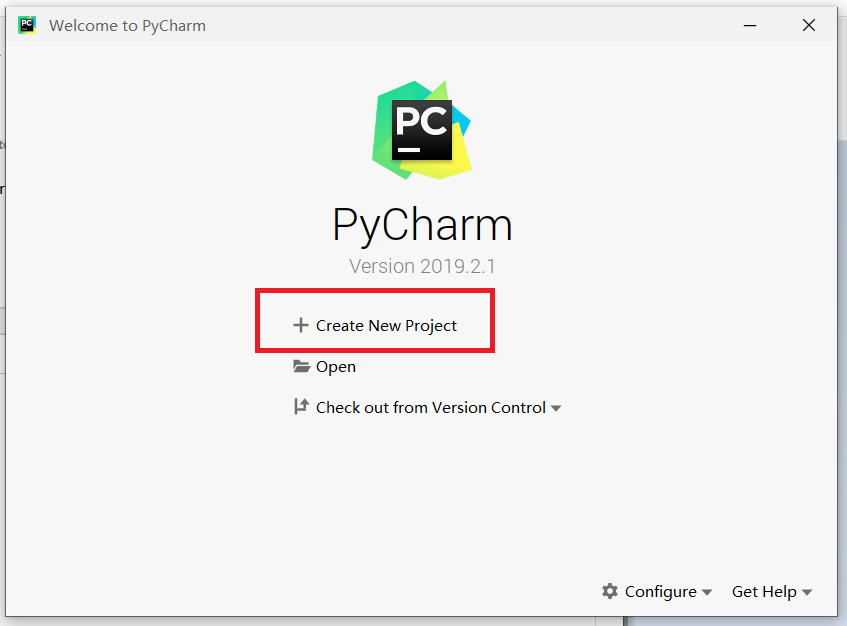
\includegraphics[scale=0.4]{figure/chapter1/pycharm13.png}\quad
  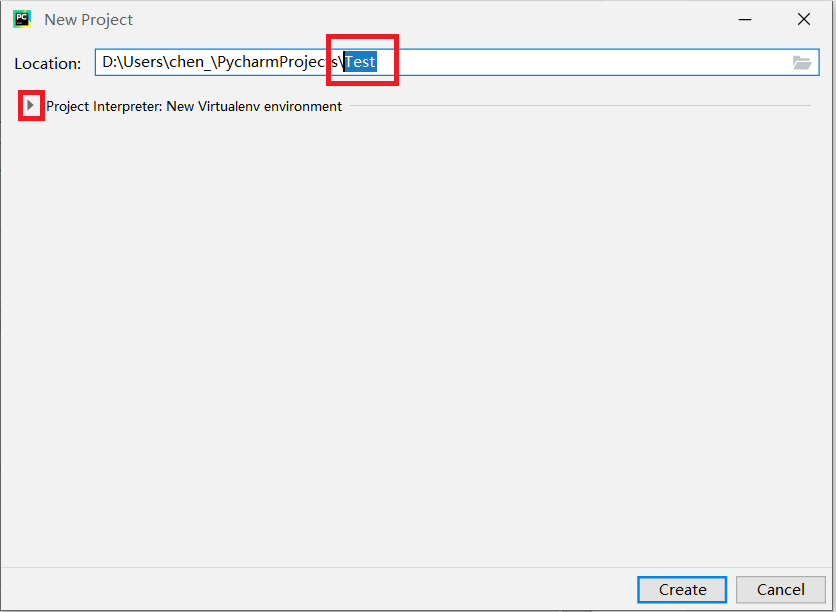
\includegraphics[scale=0.4]{figure/chapter1/pycharm14.png}
\end{figure}

% 点击这个三角符号,可以看到 Pycharm 已经自动获取了我们安装的 Python 版本。
%
%


为了测试 Pycharm 是能安装成功,可以点击 Pycharm 界面最下面的 Python Console,打开控制台(Python Console 是一个交互式的 python 编辑器,可以快速运行一些指令,一般调试时用),输入一条 Python 指令:print(`Hello World'),若能正确运行,则表示 Pycharm 安装成功了。

\clearpage

\begin{figure}[!ht]
  \centering
  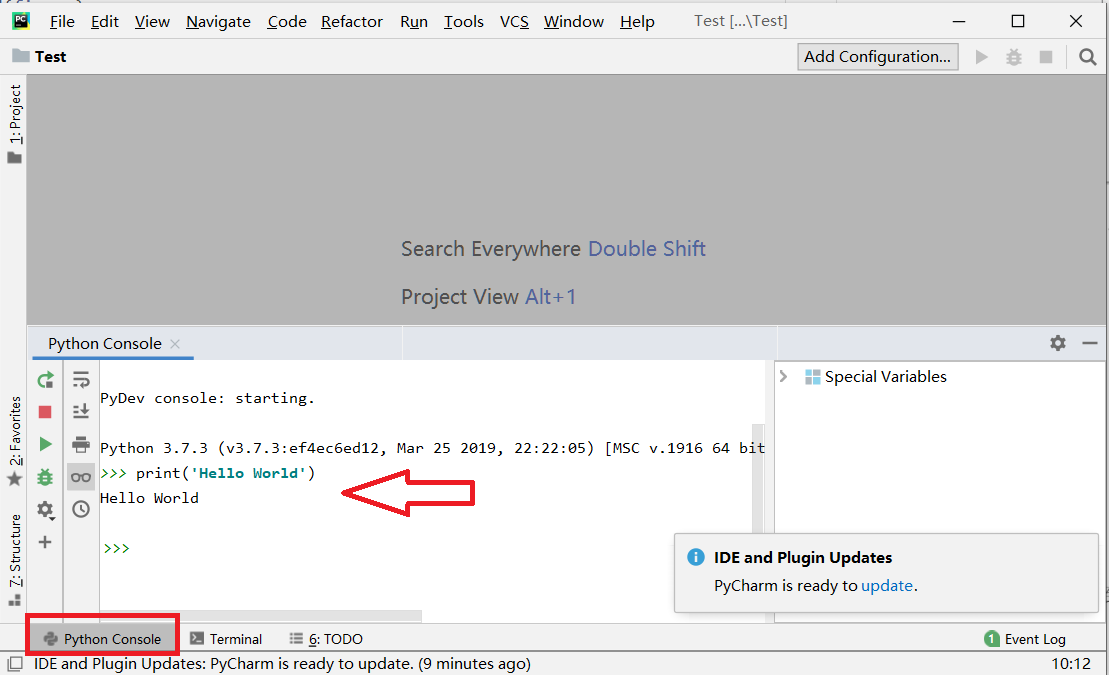
\includegraphics[scale=0.4]{figure/chapter1/pycharm4.png}
\end{figure}

有时候可能提醒我们设置 Pycharm 中的 Python 解释器。设置方式如下:依次点击 file--settings--project interpreter,将 interpreter 设置为我们 Python 安装路径中的 python.exe(笔者电脑的位置为 \path{D:\python:\python.exe})。

\begin{figure}[!ht]
  \centering
  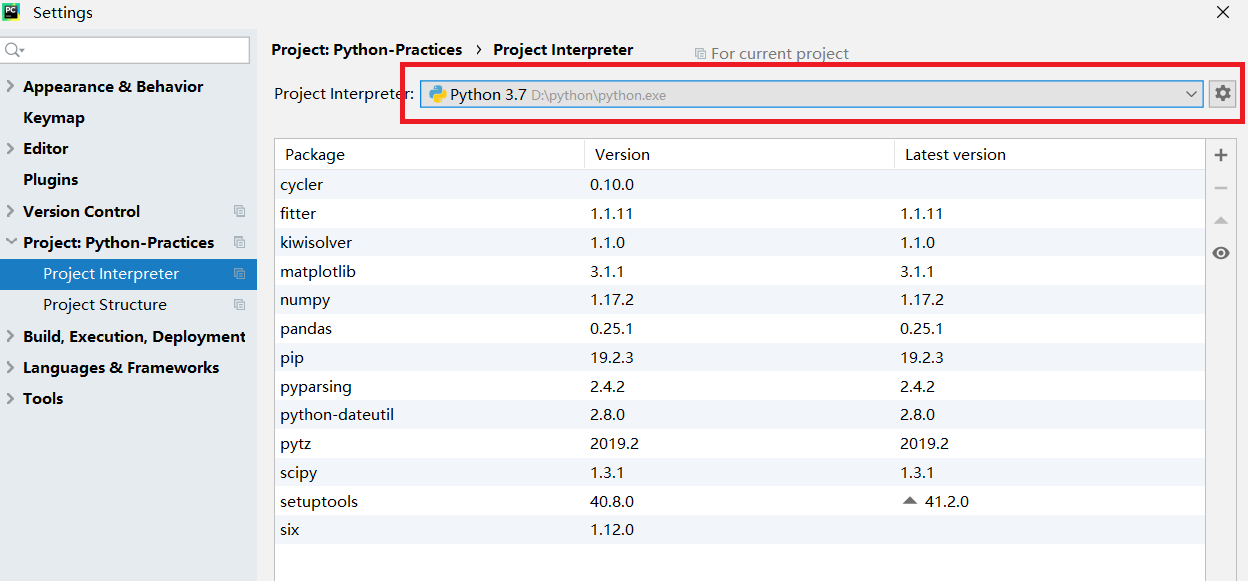
\includegraphics[scale=0.4]{figure/chapter1/pycharm3.png}
\end{figure}

我们可以在刚刚新建的项目(project)中新建一个 Python 文件,操作步骤如下图所示:

\begin{figure}[!ht]
  \centering
  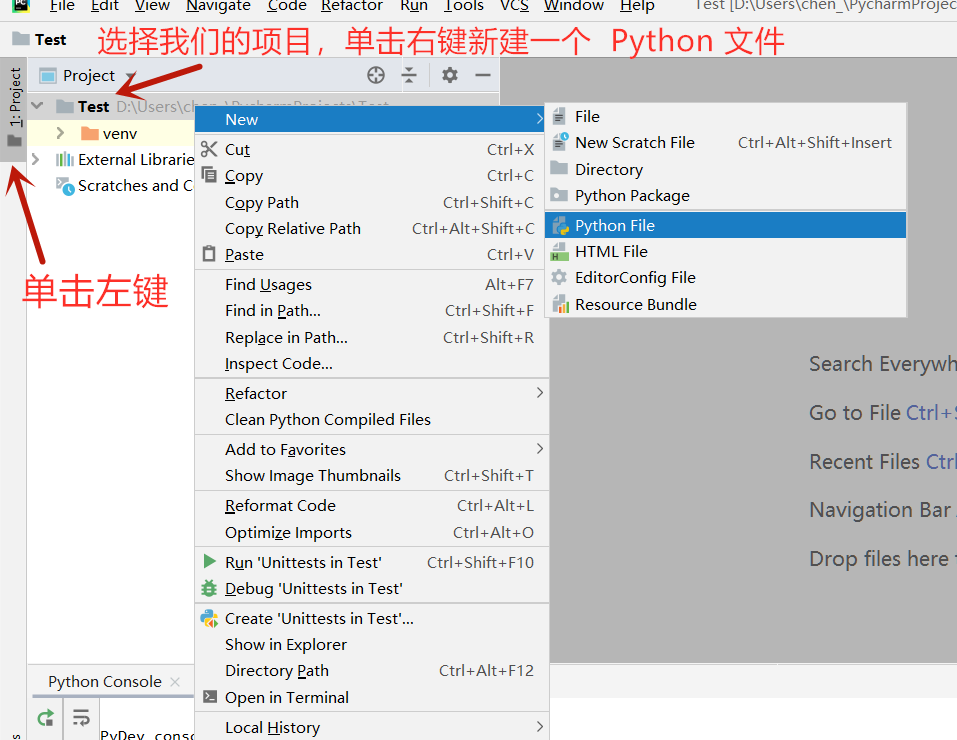
\includegraphics[scale=0.5]{figure/chapter1/pycharm15.png}
\end{figure}

命名 Python 文件的名字:

\begin{figure}[!ht]
  \centering
  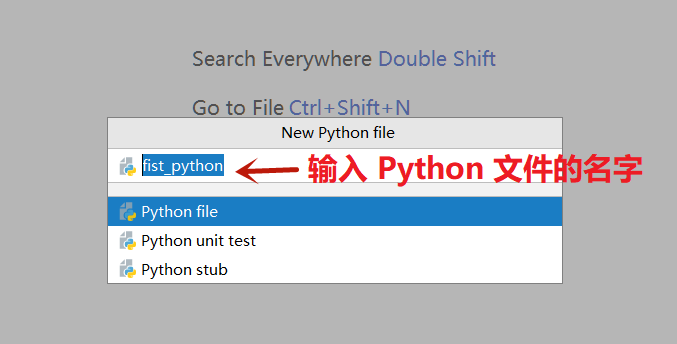
\includegraphics[scale=0.6]{figure/chapter1/pycharm16.png}
\end{figure}

输入代码后,在空白处单击右键,选择 run 运行程序:

\begin{figure}[!ht]
  \centering
  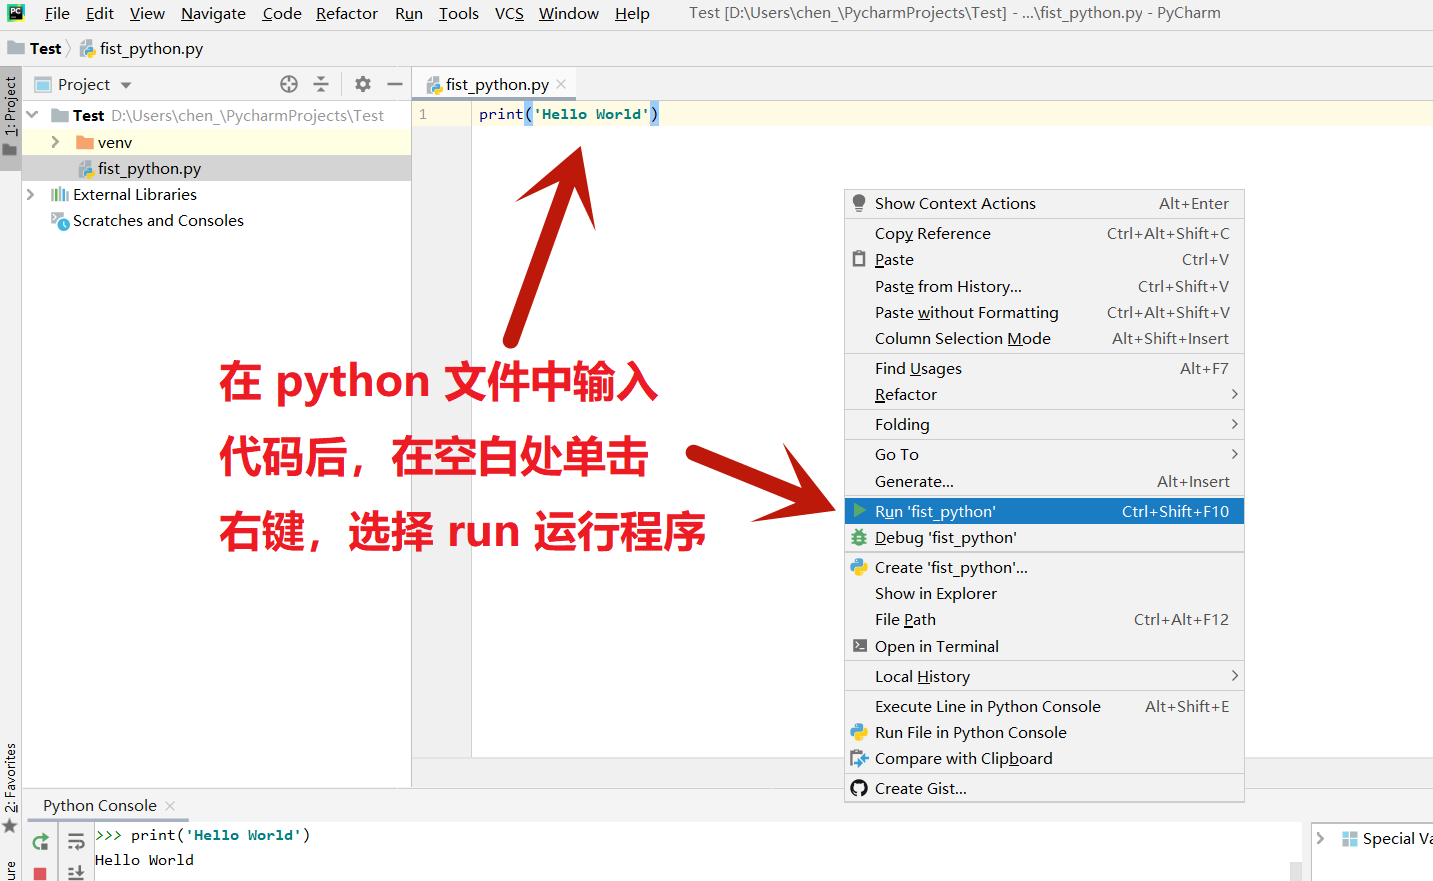
\includegraphics[scale=0.4]{figure/chapter1/pycharm17.png}
\end{figure}

在 Pycharm 下面的窗口中,就能看到运行输出的文字:

\begin{figure}[!ht]
  \centering
  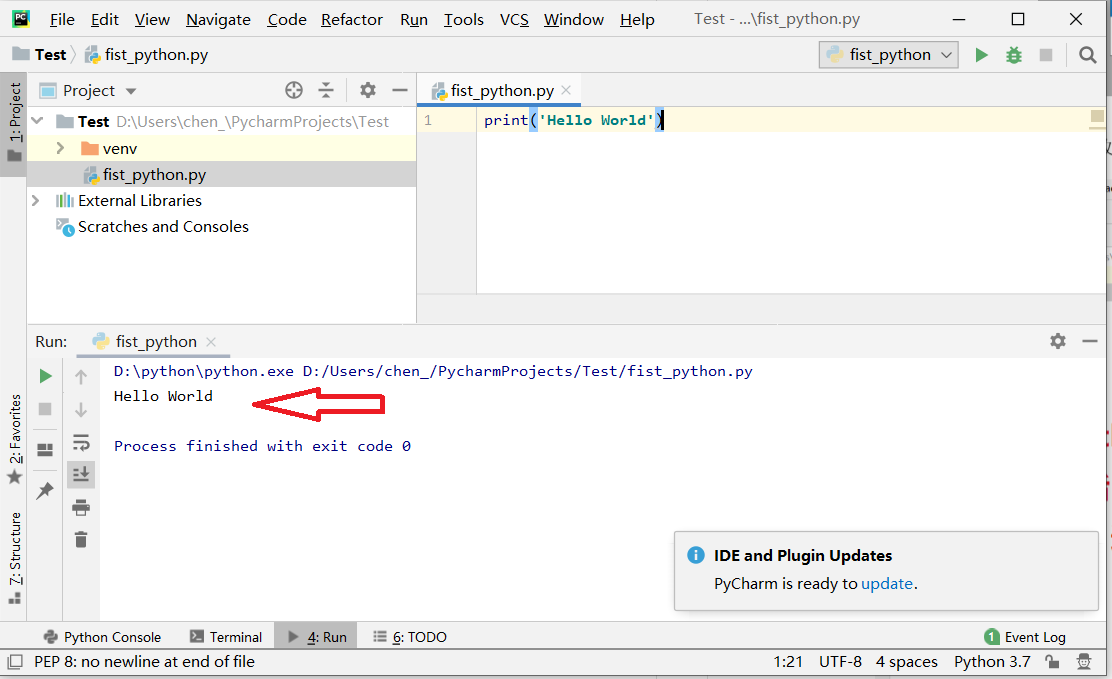
\includegraphics[scale=0.5]{figure/chapter1/pycharm18.png}
\end{figure}

\clearpage
\section{统计学常用 Python 工具包的安装}

Python 的最大优势在于它有很多第三方开发的包,能够实现各种各样的功能。若我们使用 Anaconda,一般可以通过 conda 工具安装。若我们使用 Pycharm,一般用 pip 工具进行安装。

统计学的常用包有:

\vspace{5pt}
\begin{itemize}
  \item numpy --- 用于数组和矩阵操作

  \item pandas --- 用于处理表格数据,数据分析的重要工具

  \item xlrd --- 用于读取 excel 数据

  \item openpyxl --- 用于存储 pandas 数据到 excel

  \item matplotlib --- 绘图包

  \item scipy --- 所有基础的科学算法,包括一些基础的统计学

  \item statsmodels --- 用于统计学建模和高级分析


  \item seaborn --- 对统计数据进行可视化

\end{itemize}
\vspace{5pt}

\subsection{用 Anaconda 安装}

Anaconda 已经默认帮我们安装了很多常用的包,很多时候并不需要我们再安装新包。若实在有必要,可以通过 Anaconda 自带的 Conda 工具安装。方法是:在 Windows 菜单栏里,点击 Anaconda Prompt,打开 Anaconda 的命令行窗口,如下图所示:

\begin{figure}[!ht]
  \centering
  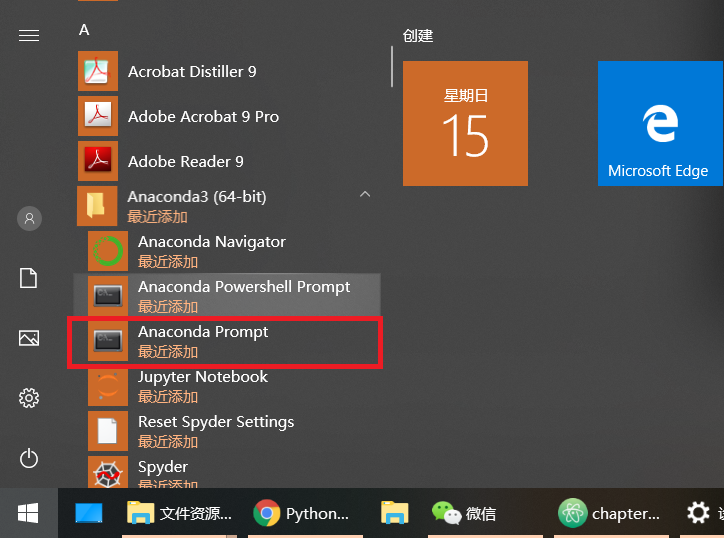
\includegraphics[scale=0.4]{figure/chapter1/anaconda6.png}
\end{figure}

常用的 conda 语法如下:

\begin{center}
\begin{tcolorbox}[title = conda 的常用语法]
  \centering\bf
  \begin{tcboutputlisting}
  \begin{tabular}{>{\bfseries}ll}
    安装包:&conda install [package\_name]\\
    搜索包:&conda search [package\_name]\\
    卸载包:&conda uninstall [package\_name]\\
    更新包: & conda install [package\_name] -U\\
  显示已安装包列表: &conda list
  \end{tabular}
\end{tcboutputlisting}
\end{tcolorbox}
\end{center}

例如,安装 numpy 包的命令输入为:conda install numpy。不过,国内用 conda 安装包时的下载网速有时候比较慢。

\subsection{用 pip 安装}
pip 是 Python 包管理工具,该工具提供了对 Python 包的查找、下载、安装、卸载的功能。在我们安装 python 时, pip 也是自动安装的,并且 pip 的地址已经添加到了计算机的环境变量里了。 打开命令行窗口(win10 系统中敲 win 健,再输入 cmd,然后回车),输入 pip (有时候若电脑里其他软件也内置 pip,则需要输入 pip.exe才能正确显示)回车,若能显示如下图所示的很多内容,则表示 pip 已经成功安装了。

\begin{figure}[!ht]
  \centering
  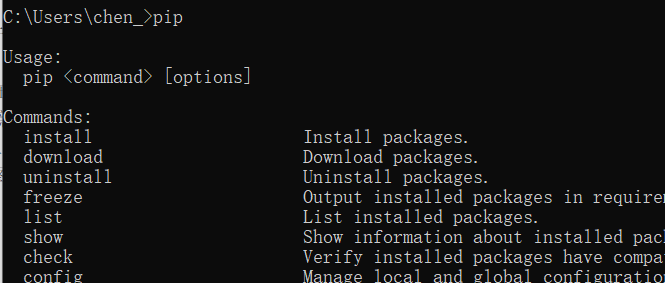
\includegraphics[scale=0.6]{figure/chapter1/pip.png}
\end{figure}

常用的 pip 语法如下:

\begin{center}
\begin{tcolorbox}[title = pip 的常用语法]
  \centering\bf
  \begin{tcboutputlisting}
  \begin{tabular}{>{\bfseries}ll}
    安装包:&pip install [package\_name]\\
    搜索包:&pip search [package\_name]\\
    卸载包:&pip uninstall [package\_name]\\
    更新包: & pip install [package\_name] -U\\
  显示已安装包列表: &pip list
  \end{tabular}
\end{tcboutputlisting}
\end{tcolorbox}
\end{center}

例如,安装 numpy 包时在命令行窗口输入 pip install numpy,操作命令与运行结果如下图。
\begin{figure}[!ht]
  \centering
  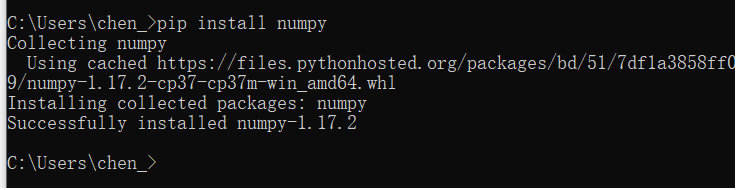
\includegraphics[scale=0.6]{figure/chapter1/pip2.png}
\end{figure}



因此,我们可以在命令行窗口,利用 pip 的安装命令将其他包安装到 Python 中。

\begin{lstlisting}
pip install pandas
pip install xlrd
pip install openyxl
pip install matplotlib
pip instal scipy
pip install statsmodels
pip install seaborn
\end{lstlisting}
